% BGIN Block 15 — the IKP co-chair's four sessions (15–16 Oct 2026, Georgetown University Capitol Campus)
% 1-4 / 1-7 PQC Migration (Room B, 15 Oct 09:50–13:00) · 2-6 Privacy Enhanced Authentication, ZKP & Proof of
% Personhood (Room B, 16 Oct 11:30–13:00) · 2-9 AML Policy, Forensics & Analytics — Common Taxonomy (FASE/IKP,
% Room A, 16 Oct 15:40–17:10, with Chloe White).
% House style of the GDC26 / Block 15 PQC decks: dark title bar, grey lead box, "Takeaway" line, BGIN mark in the footer.
% Facts follow the Block 15 programme (bgin-global.org/events/20261015-block15), bgin-global/pqc-agility-competition
% (draft v0, main 86c780a), the Block 14 meeting reports, the proof-of-human convergence note (Aug 2026) and the
% IKP KB in ~/BGIN_IKP. Everything shown is unratified.
% Build: latexmk -pdf Block15_IKP_CoChair_Sessions.tex
\documentclass[aspectratio=169,10pt]{beamer}
\usepackage[utf8]{inputenc}
\usepackage[T1]{fontenc}
\usepackage{helvet}
\renewcommand{\familydefault}{\sfdefault}
\usepackage{booktabs}
\usepackage{array}
\usepackage{graphicx}
\usepackage{fontawesome5}
\usepackage{tikz}
\usetikzlibrary{arrows.meta,positioning,calc}
\usepackage{qrcode}
\usepackage{hyperref}

\usetheme{default}
\setbeamersize{text margin left=7mm,text margin right=7mm}
\setlength{\tabcolsep}{4pt}
\definecolor{bar}{RGB}{25,25,29}
\definecolor{ink}{RGB}{35,35,40}
\definecolor{soft}{RGB}{110,110,118}
\definecolor{boxbg}{RGB}{242,242,244}
\definecolor{lane}{RGB}{225,227,232}
\definecolor{pqc}{RGB}{247,147,26}
\definecolor{pop}{RGB}{92,74,140}
\definecolor{popbg}{RGB}{236,233,244}
\definecolor{aml}{RGB}{18,108,108}
\definecolor{amlbg}{RGB}{228,240,239}
\setbeamercolor{normal text}{fg=ink}
\setbeamercolor{structure}{fg=bar}
\setbeamercolor{frametitle}{bg=bar,fg=white}
\setbeamercolor{block body}{bg=boxbg,fg=ink}
\setbeamercolor{pop body}{bg=popbg,fg=ink}
\setbeamercolor{aml body}{bg=amlbg,fg=ink}
\setbeamertemplate{navigation symbols}{}
\setbeamertemplate{itemize item}{\color{bar}\faAngleRight}
\setbeamertemplate{itemize subitem}{\color{soft}\textendash}
\setbeamertemplate{enumerate item}{\colorbox{bar}{\color{white}\scriptsize\insertenumlabel}}
\setbeamerfont{frametitle}{series=\bfseries,size=\large}
\setbeamertemplate{frametitle}{%
  \vskip-2pt\begin{beamercolorbox}[wd=\paperwidth,ht=8mm,dp=2.5mm,leftskip=6mm]{frametitle}%
  \usebeamerfont{frametitle}\insertframetitle\hfill{\small\mdseries\insertframesubtitle}\hspace{6mm}\end{beamercolorbox}}
\setbeamertemplate{footline}{%
  \begin{beamercolorbox}[wd=\paperwidth,ht=5mm,dp=2mm,leftskip=6mm,rightskip=6mm]{normal text}%
  \tiny\color{soft}\raisebox{-1.2pt}{
\includegraphics[height=3.2mm]{bgin_mark.png}}\hspace{1.2mm}%
  BGIN Block 15 --- IKP 2-6: Privacy Enhanced Authentication, ZKP \& Proof of Personhood\hfill Washington, D.C. \textbar{} 16 Oct 2026, 11:30 / \insertframenumber\end{beamercolorbox}}
\newcommand{\takeaway}[1]{\par\vspace{1.5mm}{\small\color{bar}\faLink~\textbf{Takeaway:} #1}}
\newcommand{\lead}[1]{\begin{beamercolorbox}[wd=\textwidth,sep=2.5mm]{block body}\small #1\end{beamercolorbox}\par\vspace{2mm}}
\newcommand{\poplead}[1]{\begin{beamercolorbox}[wd=\textwidth,sep=2.5mm]{pop body}\small #1\end{beamercolorbox}\par\vspace{2mm}}
\newcommand{\amllead}[1]{\begin{beamercolorbox}[wd=\textwidth,sep=2.5mm]{aml body}\small #1\end{beamercolorbox}\par\vspace{2mm}}
\newcommand{\pillar}[3]{\begin{minipage}[t]{#1}\colorbox{bar}{\parbox{\dimexpr\linewidth-2\fboxsep}{\color{white}\small\textbf{#2}}}\par\vspace{1mm}{\small #3}\end{minipage}}
\newcommand{\cpillar}[4]{\begin{minipage}[t]{#2}\colorbox{#1}{\parbox{\dimexpr\linewidth-2\fboxsep}{\color{white}\small\textbf{#3}}}\par\vspace{1mm}{\small #4}\end{minipage}}
% \sectiontitle{accent}{kicker}{title}{subtitle}
\newcommand{\sectiontitle}[4]{{\setbeamertemplate{footline}{}\begin{frame}[plain]
  \begin{tikzpicture}[remember picture,overlay]
    \fill[bar] (current page.north west) rectangle (current page.south east);
    \node[anchor=north east,inner sep=0] at ([xshift=-7mm,yshift=-5mm]current page.north east){
\includegraphics[height=1.9cm]{bgin_logo.png}};
    \node[anchor=south west,text=#1,font=\small\bfseries] at ([xshift=7mm,yshift=-2.9cm]current page.north west){#2};
    \node[anchor=south west,text=white,font=\Large\bfseries,text width=13cm,align=left] at ([xshift=7mm,yshift=-4.7cm]current page.north west){#3};
    \node[anchor=north west,text=white,font=\small,text width=13cm,align=left] at ([xshift=7mm,yshift=-5.0cm]current page.north west){#4};
  \end{tikzpicture}
\end{frame}}}
\hypersetup{colorlinks,urlcolor=bar,linkcolor=ink}
\newcommand{\nohyph}{\hyphenpenalty=10000 \exhyphenpenalty=10000 \relax}

\begin{document}

% ================================================================ TITLE
{\setbeamertemplate{footline}{}
\begin{frame}[plain,t]
  \begin{tikzpicture}[remember picture,overlay]
    \fill[bar] (current page.north west) rectangle ([yshift=-3.5cm]current page.north east);
    \node[anchor=north east,inner sep=0] at ([xshift=-7mm,yshift=-5mm]current page.north east){
\includegraphics[height=1.9cm]{bgin_logo.png}};
    \node[anchor=west,text=white,font=\Large\bfseries,text width=11.2cm,align=left] at ([xshift=7mm,yshift=-1.35cm]current page.north west){Privacy Enhanced Authentication, ZKP \& Proof of Personhood};
    \node[anchor=west,text=pop,font=\small,text width=11.2cm,align=left] at ([xshift=7mm,yshift=-2.85cm]current page.north west){IKP session 2-6 \textperiodcentered{} authentication that proves the claim without disclosing the person};
    \node[anchor=west,font=\normalsize,text width=13.2cm] at ([xshift=7mm,yshift=-4.6cm]current page.north west){Mitchell Travers (chair) \textperiodcentered{} World as main discussant \textperiodcentered{} contributors to the IKP proof-of-personhood paper};
    \node[anchor=north west,font=\small,text=soft,text width=13.2cm,align=left] at ([xshift=7mm,yshift=-5.0cm]current page.north west){BGIN Block \#15 \textbar{} Georgetown University Capitol Campus, Washington, D.C. \textbar{} 16 October 2026, Room B, 11:30--13:00, then the World lunch session 13:00--14:00 \textbar{} hybrid};
    \node[anchor=west,font=\scriptsize,text=soft,text width=13cm,align=left] at ([xshift=7mm,yshift=-6.5cm]current page.north west){Builds on the Block 14 reports \emph{Privacy Enhanced Authentication and Key Management} and \emph{Proof of Personhood} and the open IKP meetings since \textperiodcentered{} disclosure: the chair also co-chairs the ToIP DTG ZKP Task Force; observations on that work are personal and from public materials};
  \end{tikzpicture}
\end{frame}}

% ================================================================ CONTEXT
\begin{frame}{This Session --- What It Is For}
  \poplead{Privacy-enhanced authentication at a high level, the proof-of-personhood taxonomy and the distinctions it has to keep, verifiable trust agents acting for a person, and where zero-knowledge proofs do the work. Twenty minutes for contributors, then open discussion into the IKP proof-of-personhood paper.}
  \begin{enumerate}\footnotesize\setlength{\itemsep}{0.5mm}
    \item Why now: agentic AI raises the cost of not knowing a counterparty is human
    \item Prove the claim, not the identity: minimal disclosure, unlinkability, what each proof proves, where the biometric lives, what revocation means when the binding cannot be rotated
    \item The taxonomy, with World as main discussant: unique human versus specific human, humanity versus uniqueness, linkability scope, strength expression, continuity, agent authority
    \item Verifiable trust agents: an agent acting for a person carrying personhood assurance with delegated scope
    \item ZKP where it earns its place: predicates that carry strength, client-side proving on everyday phones, post-quantum readiness of the stack
    \item Contributions (20 min); then the gaps nobody owns yet; then next steps into the paper, public comment, and the ISO TC 307 Technical Report path
  \end{enumerate}
  \takeaway{Leave with room comments on the paper's structure, a contributor list, and the unclaimed gaps confirmed as IKP's contribution.}
\end{frame}

% ================================================================ 17 why now
\begin{frame}{Why Now --- Agentic AI Raises the Cost of Not Knowing}
  \poplead{When an AI system rather than a person can hold a wallet, pay, post and transact, every counterparty has to ask a question that used to be free: \textbf{is there a human here, and on whose authority is this agent acting?} The answer must not cost the human their privacy.}
  \begin{columns}[T]
    \begin{column}{0.48\textwidth}
      {\small\textbf{Block 14 left two reports}}
      \begin{itemize}\small
        \item \emph{Privacy Enhanced Authentication and Key Management}: one system holds the keys, another composes the transactions; AI as a separate process from the key holder, with scoped, revocable access
        \item \emph{Proof of Personhood}: the three-graph model, the dual-agent separation, the human stack, and the ISO TC 307 Technical Report path --- Block 15 named for public comment
      \end{itemize}
    \end{column}
    \begin{column}{0.48\textwidth}
      {\small\textbf{Since then}}
      \begin{itemize}\small
        \item IKP research pathway on ZK proofs for biometric authentication (July); open, topic-focused IKP meetings on the taxonomy
        \item A working note mapping three converging efforts: World's Proof of Human framework, the ToIP DTG credential and proof-of-liveness work, this paper
        \item Client-side ZK proving on everyday phones became real (ProveKit)
      \end{itemize}
    \end{column}
  \end{columns}
  \takeaway{The question is no longer whether personhood can be proven privately, but what a given proof proves, and to whom.}
\end{frame}

% ================================================================ 18 prove the claim
\begin{frame}{Prove the Claim, Not the Identity}
  \cpillar{pop}{0.31\textwidth}{What each proof proves}{Proof of \emph{a} human (uniqueness) is not proof of \emph{a specific} human (identity). A relying party should be told which one it is getting, at what strength, against which adversary --- and what the proof explicitly does not establish.}\hfill
  \cpillar{pop}{0.31\textwidth}{Where the biometric lives}{On the device, signed by the capture hardware and held by the person; uniqueness checked without an identity lookup (sMPC in World's design); government ID matched locally if at all. The architecture decides the harm if it fails.}\hfill
  \cpillar{pop}{0.31\textwidth}{Revocation of what cannot rotate}{A key can be rotated. An iris cannot. Revocation for a credential bound to a biometric means revoking the \emph{binding} and the \emph{enrolment}, not the person --- and saying so in the taxonomy.}
  \par\vspace{2.5mm}
  {\small Minimal disclosure and unlinkability are the two privacy properties every pattern here is scored on. Verifiability is not truth: a proof can be perfectly verifiable and still establish less than the relying party assumes.}
  \takeaway{A taxonomy that cannot say which of these a scheme delivers cannot be used to certify one.}
\end{frame}

% ================================================================ 19 the layers
\begin{frame}{Three Efforts, One Stack --- the Convergence Map}
  \poplead{Three efforts converged on the same structure independently. The friction is almost entirely at the seams between layers, which is where a working group earns its keep.}
  \begin{center}\scriptsize
  \begin{tabular}{@{}p{3.3cm}p{5.6cm}p{4.9cm}@{}}\toprule
    \textbf{Layer} & \textbf{Question it answers} & \textbf{Who is working here}\\ \midrule
    Assurance semantics & What class of claim, at what strength, on what evidence; how it maps to NIST xAL and ISO 29115 & World \emph{Proof of Human} framework (v0.13, Aug 2026: ten categories, four dimensions)\\
    Predicate semantics & What a proof establishes, what it does \emph{not}, what it discloses, to whom, against which adversary, for how long & ToIP DTG ZKP Task Force, proof-of-liveness requirements v0.4\\
    Mechanism & Which credential, protocol and proof construction carries the claim & DTG Core Credentials WD01; First Person Network\\
    Formal security & What the claim provably guarantees against a defined adversary & \emph{A Cryptographic Framework for Proof of Personhood} (ePrint 2026/333)\\
    Governance \& policy & Who may assert this, in what domain, under what regulatory consequence & \textbf{BGIN IKP}; trust registries; ISO TC 307\\ \bottomrule
  \end{tabular}
  \end{center}
  {\scriptsize\color{soft} Disclosure: the chair also co-chairs the ToIP DTG ZKP Task Force; observations on that work are personal and drawn from public materials.}
  \takeaway{Published standalone, a new taxonomy is a fourth competing vocabulary. Published as a layer bound to the predicates beneath it, it is what makes the others interoperable.}
\end{frame}

% ================================================================ 20 five distinctions
\begin{frame}{Five Distinctions the Taxonomy Has to Keep}
  \begin{center}\small
  \begin{tabular}{@{}p{3.0cm}p{10.8cm}@{}}\toprule
    \textbf{Distinction} & \textbf{Why it is load-bearing}\\ \midrule
    Humanity $\neq$ uniqueness & Two different claims, routinely collapsed into one credential. Liveness plus presence plus absence-of-automation is not the same as ``one person, once, in this domain''.\\
    Linkability scope & Adopt the architecture (pairwise, domain-scoped, global), then parameterise the dimension. A uniqueness assertion that survives across domains is a correlation key.\\
    Strength expression & The headline gap: how assurance is \emph{stated} rather than asserted --- ordinal scale, per-category scale, or a profile-defined vector a relying party can actually consume.\\
    Continuity & Continuity with enrolment is a property of the carrier and its controls, not of the primitive. Enrolment poisoning is its adversary.\\
    Agent authority & An agent acting for a human: the field list exists in the credential work; it needs completing with scope, delegation and revocation.\\ \bottomrule
  \end{tabular}
  \end{center}
  \takeaway{World is the main discussant here because its framework is strongest on strength expression and on separating humanity from uniqueness --- the two places the existing standards are thinnest.}
\end{frame}

% ================================================================ 21 three graphs + dual agent
\begin{frame}{The Block 14 Model --- Three Graphs, Two Agents}
  \begin{center}
  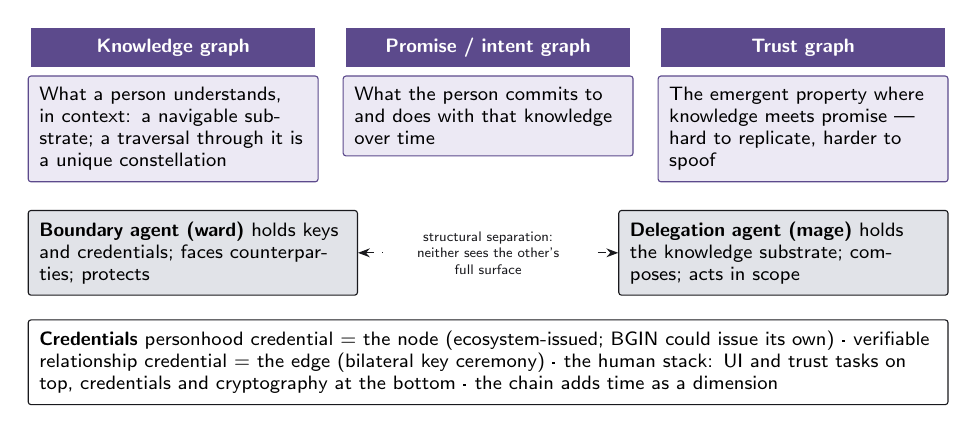
\begin{tikzpicture}[font=\scriptsize, g/.style={draw=pop,fill=popbg,rounded corners=1pt,text width=3.4cm,align=left,inner sep=4pt}, hd/.style={fill=pop,text=white,font=\scriptsize\bfseries,text width=3.4cm,align=center,inner sep=3pt,minimum height=5mm}, a/.style={draw=bar,fill=lane,rounded corners=1pt,text width=3.9cm,align=left,inner sep=4pt}]
    \node[hd] (h1) at (0,0) {Knowledge graph};
    \node[hd] (h2) at (4.0,0) {Promise / intent graph};
    \node[hd] (h3) at (8.0,0) {Trust graph};
    \node[g,below=1mm of h1] (g1) {What a person understands, in context: a navigable substrate; a traversal through it is a unique constellation};
    \node[g,below=1mm of h2] (g2) {What the person commits to and does with that knowledge over time};
    \node[g,below=1mm of h3] (g3) {The emergent property where knowledge meets promise --- hard to replicate, harder to spoof};
    \node[a,anchor=north west] (s) at ([yshift=-3.5mm]g1.south west) {\textbf{Boundary agent (ward)} holds keys and credentials; faces counterparties; protects};
    \node[a,anchor=north east] (m) at ([yshift=-3.5mm]g3.south east) {\textbf{Delegation agent (mage)} holds the knowledge substrate; composes; acts in scope};
    \draw[{Stealth[length=1.5mm]}-{Stealth[length=1.5mm]},bar,dashed] (s.east) -- node[font=\tiny,align=center,text width=2.6cm,fill=white,inner sep=1pt]{structural separation:\\ neither sees the other's\\ full surface} (m.west);
    \node[draw=bar,fill=white,rounded corners=1pt,text width=11.4cm,inner sep=4pt,align=left,anchor=north] at ([yshift=-3mm]$(s.south)!0.5!(m.south)$) {\textbf{Credentials} personhood credential = the node (ecosystem-issued; BGIN could issue its own) \textperiodcentered{} verifiable relationship credential = the edge (bilateral key ceremony) \textperiodcentered{} the human stack: UI and trust tasks on top, credentials and cryptography at the bottom \textperiodcentered{} the chain adds time as a dimension};
  \end{tikzpicture}
  \end{center}
  \takeaway{The knowledge substrate never touches the wallet. The person is proven at the overlap of what they know, what they promise, and the trust that emerges between two agents that cannot fully see each other.}
\end{frame}

% ================================================================ 22 verifiable trust agents
\begin{frame}{Verifiable Trust Agents --- Personhood with Delegated Scope}
  \poplead{An agent acting for a person can carry personhood assurance with a declared scope. The question for the taxonomy: does the principal need to be \emph{identified}, or only \emph{assured as human} with delegated authority?}
  \begin{columns}[T]
    \begin{column}{0.5\textwidth}
      {\small\textbf{What the agent carries}}
      \begin{itemize}\small
        \item A personhood credential as the node; relationship credentials as the edges it may traverse
        \item Delegation scope: what it may read, what it may share, on whose authority, until when
        \item Revocation that reaches the delegation, not the person
      \end{itemize}
    \end{column}
    \begin{column}{0.47\textwidth}
      {\small\textbf{The written contribution to this Block}}
      \begin{itemize}\small
        \item \emph{Separation of Duties for Personal AI Agents} (discussion paper proposing a work item): two agents with disjoint duties and structural context erasure between them
        \item Separation classified by \textbf{reachability}, not by rule: policy-enforced if some permitted sequence can reconstruct the shared origin; structural if none can
        \item Deliverables: a documentation profile under which every separation claim names its preconditions, adversary class and date. Eight open questions, none asserted.
      \end{itemize}
    \end{column}
  \end{columns}
  \takeaway{The same principle as the Block 14 key-management report and as session 2-8 this afternoon: one system holds the keys, another composes the transactions.}
\end{frame}

% ================================================================ 23 ZKP where it earns its place
\begin{frame}{Zero-Knowledge Proofs Where They Earn Their Place}
  \cpillar{pop}{0.31\textwidth}{Predicates that carry strength}{A proof should disclose the assurance class and policy identifier without leaking the issuer. Open: whether issuer--verifier collusion resistance is achievable at all once schema rarity, status traffic and timing are counted.}\hfill
  \cpillar{pop}{0.31\textwidth}{Proving on the phones people own}{ProveKit (World, Atheon, Reilabs, Nethermind): Noir circuits proven on-device, verified on chain or in a browser. iPhone SE 3: 2--3 s; 2 GB Android: under 30 s; under 500 MB peak memory. ``Trusted setup is a distribution problem before it is a trust problem.''}\hfill
  \cpillar{pop}{0.31\textwidth}{Post-quantum readiness of the stack}{Personhood credentials, relationship credentials and ZK proofs over biometrics all rest on primitives in the PQC migration's scope. Lattice-based proof systems are arriving; the credential stack has to be migratable, not just the signatures.}
  \par\vspace{2.5mm}
  {\small Not a ZKP-only session: the proof layer is one row of the stack. It does the work only where the predicate it proves has been written down with its negative space --- what it does not establish.}
  \takeaway{``PQC-ready'' and ``privacy-preserving'' are the same kind of claim: testable only against a published definition. Thursday's register and today's taxonomy are two halves of that definition.}
\end{frame}

% ================================================================ 24 gaps nobody owns
\begin{frame}{Gaps Nobody Owns --- Candidate IKP Work Items}
  \begin{center}\scriptsize
  \begin{tabular}{@{}p{3.3cm}p{10.5cm}@{}}\toprule
    \textbf{Gap} & \textbf{Why it is BGIN's}\\ \midrule
    Coercion, duress, credential rental & A human can be present, live, unique and cryptographically flawless --- and still a rented proxy. Fencing it off as ``not established'' is not treatment. Governance and economics more than cryptography.\\
    Threat model per assurance category & Sybil (uniqueness) \textperiodcentered{} injection and deepfake (presence) \textperiodcentered{} enrolment poisoning (continuity) \textperiodcentered{} credential theft (control) \textperiodcentered{} duress (action) \textperiodcentered{} farming. ISO SC 27 needs the adversary column; the drafting discipline exists, its application does not.\\
    Governance of the domain & ``Unique within a declared domain'' needs someone authorised to declare and govern it. Who accredits a context authority? What happens when two disagree about the same human? Appeal when a human is falsely denied.\\
    Regulatory interface & An unlinkable-by-design personhood credential and a sanctions-screening duty that presumes identifiability are on a collision course. Neither ToIP nor World will write this. Session 2-9 this afternoon is where it lands.\\
    Global registry harms & A uniqueness assertion that survives across domains is a correlation key: exclusion, state coercion, irreversible biometric enrolment, function creep.\\ \bottomrule
  \end{tabular}
  \end{center}
  \takeaway{Unclaimed across both ToIP workstreams, unaddressed by NIST, squarely in BGIN's competence. The paper takes them as its contributed section.}
\end{frame}

% ================================================================ 25 discussion
\begin{frame}{Session 2-6 --- Discussion Items}
  \begin{enumerate}\small
    \item Should assurance strength be a \textbf{single ordinal scale}, per-category scales, or a profile-defined vector? What does a relying party actually consume?
    \item Is ``humanity'' a \textbf{primitive claim}, or the union of liveness, presence and absence-of-automation? Is the third even provable? If it decomposes, strength attaches per component.
    \item For \textbf{agent authority}: does the human principal need to be identified, or only assured as human with delegated scope?
    \item How does any personhood claim survive \textbf{coercion and credential rental} --- and if it cannot, how should the taxonomy say so?
    \item Who \textbf{accredits a context authority}, what is the appeal path when a human is falsely denied uniqueness, and who supervises?
  \end{enumerate}
  \par\vspace{1mm}
  {\small Every answer in the form the predicate work already uses: every parameter bound, adversary and horizon declared, negative space written.}
\end{frame}

% ================================================================ 26 next steps
\begin{frame}{Session 2-6 --- Where It Goes}
  \poplead{Room comments go into the IKP proof-of-personhood paper; the paper goes out for public comment; the standards path is an ISO TC 307 Technical Report --- a survey of the state of the world, one voting round, not a four-year International Standard.}
  \begin{columns}[T]
    \begin{column}{0.48\textwidth}
      {\small\textbf{The paper}}
      \begin{itemize}\small
        \item Three-graph model and dual-agent separation (Block 14)
        \item Assurance decomposition as a contributed section; the convergence mapping as an annex
        \item The unclaimed gaps as the BGIN-specific contribution
        \item PQC migration of the credential stack as a requirement, not an afterthought
      \end{itemize}
    \end{column}
    \begin{column}{0.48\textwidth}
      {\small\textbf{The afternoon}}
      \begin{itemize}\small
        \item 13:00--14:00, Room B --- lunch session with World: proof of a unique human in practice, and the client-side ZK tooling behind it; questions from the room feed the taxonomy
        \item 14:00--14:45, Room B --- Offline Key Management (Cyber + IKP): the same separation principle, applied to cold storage
        \item 15:40--17:10, Room A --- the regulatory interface, next
      \end{itemize}
    \end{column}
  \end{columns}
  \takeaway{Bring something half-built from real implementation to the standards body; do not start from scratch in committee. The room's job is to make the half-built thing honest.}
\end{frame}

% ================================================================ ENGAGE
\begin{frame}{How to Engage}
  \begin{columns}[T]
    \begin{column}{0.55\textwidth}
      \begin{itemize}\small
        \item \textbf{Read} the two Block 14 meeting reports on the Privacy Enhanced Authentication hub.
        \item \textbf{Add research questions} to the ZKP / biometric authentication pathway thread on the IKP Discourse.
        \item \textbf{Join} the open, topic-focused IKP meetings on the taxonomy between Blocks.
        \item \textbf{Comment} on the proof-of-personhood paper when it is released for public comment; contributors are credited in it.
        \item \textbf{Stay} for the lunch session with World, 13:00 in this room: proof of a unique human in practice, and the client-side ZK tooling behind it.
      \end{itemize}
    \end{column}
    \begin{column}{0.42\textwidth}
      \begin{center}\tiny
        \begin{tabular}{@{}>{\centering\arraybackslash}p{1.85cm}@{\hspace{1mm}}>{\centering\arraybackslash}p{1.85cm}@{\hspace{1mm}}>{\centering\arraybackslash}p{1.85cm}@{}}
          \qrcode[height=1.35cm]{https://bgin-global.org/events/20261015-block15/sessions/2-6} &
          \qrcode[height=1.35cm]{https://bgin-global.org/projects/privacy-enhanced-auth} &
          \qrcode[height=1.35cm]{https://bgin.discourse.group} \\[0.5mm]
          \textbf{This session} & \textbf{Project hub} & \textbf{BGIN Discourse} \\
          bgin-global.org/events/ 20261015-block15/sessions/2-6 & bgin-global.org/projects/ privacy-enhanced-auth & bgin.discourse.group
        \end{tabular}
      \end{center}
    \end{column}
  \end{columns}
  \takeaway{The paper goes out for public comment after this Block; the room's comments decide what it says about strength, uniqueness and agent authority.}
\end{frame}

% ================================================================ CLOSE
{\setbeamertemplate{footline}{}
\begin{frame}[plain]
  \begin{tikzpicture}[remember picture,overlay]
    \fill[bar] (current page.north west) rectangle (current page.south east);
    \node[anchor=south,text=white,font=\Large\bfseries,text width=13.5cm,align=center,execute at begin node=\nohyph] at ([yshift=6mm]current page.center){Prove the claim, not the identity.};
    \node[anchor=north,text=white,font=\small,text width=13.5cm,align=center,execute at begin node=\nohyph] at ([yshift=3mm]current page.center){The person is proven at the overlap: what they know, what they promise, and the trust that emerges between two agents that can never fully see each other.};
    \node[anchor=north,text=soft,font=\small,text width=13.5cm,align=center,execute at begin node=\nohyph] at ([yshift=-9mm]current page.center){BGIN IKP Working Group \textperiodcentered{} Privacy Enhanced Authentication hub on bgin-global.org \textperiodcentered{} bgin.discourse.group};
    \node[anchor=south east,inner sep=0] at ([xshift=-7mm,yshift=5mm]current page.south east){
\includegraphics[height=1.4cm]{bgin_logo.png}};
  \end{tikzpicture}
\end{frame}}

\end{document}
